\documentclass[12pt]{article}

% ---------------------------------------------------------------------------
% Political Analysis Research Article submission.
% Word budget: <=6,000 words (abstract + body + figure legends + footnotes;
% title page, references, and table-cell content excluded).
% Political Analysis uses single-ANONYMOUS review: the author is NOT
% anonymized to reviewers (only the reverse). Author identity belongs on
% this manuscript's own first page -- do not strip it into a separate file.
% Citation style: Chicago author-date (natbib + chicago.bst).
% ---------------------------------------------------------------------------
\usepackage{fontspec}
\usepackage{microtype}
\usepackage[margin=1in]{geometry}
\usepackage{graphicx}
\usepackage{amsmath}
\usepackage{booktabs}
\usepackage{array}
\usepackage{caption}
\usepackage{float}
\usepackage{setspace}
\usepackage[colorlinks=true, linkcolor=black, citecolor=black, urlcolor=blue]{hyperref}
\usepackage{xurl}
\usepackage[authoryear,round]{natbib}
\bibpunct{(}{)}{;}{a}{}{,}

\doublespacing
\setlength{\parindent}{0pt}
\setlength{\parskip}{0.6em}

\begin{document}

% =============================================================================
% Title page (first page of the manuscript itself -- not a separate file)
% =============================================================================
\begin{center}
{\LARGE\textbf{An error budget for political-bias measurement in large
language models}}

\vspace{1.5em}
{\large Sachin Letchumanan}\\[2pt]
\href{https://orcid.org/0009-0002-2216-4252}{ORCID: 0009-0002-2216-4252}

\vspace{0.5em}
Virginia Tech

\vspace{0.5em}
\textit{Corresponding author:} Sachin Letchumanan,
\href{mailto:sachin.letchumanan@gmail.com}{sachin.letchumanan@gmail.com}
\end{center}

\vspace{1em}
\begin{abstract}
\noindent
Large language models are widely reported to lean left of centre, replicated
across dozens of studies. We show this is substantially a property of
measurement. Administering the Political Compass and 8Values to 19 models,
60 times each (2,280 administrations), we decompose a measured political
position into variance from model identity, instrument choice, and trial
noise. Instrument and axis choice accounts for 52\% of variance (95\% CI
[35\%, 72\%]) and model identity for only 13\% ([0.02\%, 22\%]): which
questionnaire an auditor picks moves a score four times more than which
model is audited. The two instruments also fail convergent validity:
$r=-0.26$ for shared constructs versus $r=+0.52$ for distinct ones on the
same instrument. Crossing two further instruments, SapplyValues and Pew's
2026 Political Typology, into the same model collapses the pooled
model-identity share to 1.89\%. Three additional factors, asker identity,
instrument contamination, and response format, each explain more variance
in their factorial designs than model identity explains under the standard
protocol. Reported bias magnitudes are therefore not comparable across
studies using different instruments, and every factor examined explains
more of a score than the model producing it does. We propose a minimum
reporting standard for such audits.
\end{abstract}

\clearpage

% =============================================================================
\section{Introduction}
% =============================================================================

Large language models now mediate political information for hundreds of
millions of people, and whether that matters depends on whether a measured
lean transfers to behaviour. There is evidence that it does: interacting
with a politically biased model shifts the policy views and voting
intentions of users who were undecided beforehand \citep{fisher2026biasedai},
models can be as persuasive as targeted human messaging on contested policy
questions \citep{bai2025persuade, hackenburg2025levers}, and merely
perceiving a model as politically biased changes how much people trust its
outputs on unrelated tasks \citep{digiuseppe2026perceived}. A measured
political lean is therefore a reasonable object of study, and auditing it
is a reasonable thing to do. A substantial literature has done exactly
that, replicated across model families, providers, and languages
\citep{rozado2024, motoki2024, hartmann2023, feng2023, buyl2026,
peng2026beyond, sakhawat2026polalign}. Rozado (2024) and Motoki et al.
(2024) established the finding on early GPT-family models using the
Political Compass; Hartmann et al. (2023) and Feng et al. (2023) extended
it across a wider model set and connected the lean to downstream generation
behaviour; Buyl et al. (2026) and Peng et al. (2026) trace it to specific
choices in pretraining data and alignment fine-tuning. All of them measure
model identity's contribution to a reported score; none quantifies it
against the contribution of the measurement apparatus itself.

Each assumption behind that apparatus has since been challenged in
isolation. Models accommodate the political identity they infer for the
asker \citep{tornberg2026sycophancy}; the instruments themselves appear in
pretraining data \citep{bianchi2026plasticity}; forced-choice framing
produces answers models do not give when responding freely
\citep{rottger2024}. This journal has itself published a Letter using the
same basic technique below, repeatedly querying an LLM and averaging, to
position political texts against expert benchmarks. Its Discussion advises
readers against skipping a validation stage the paper does not itself
perform \citep{lemens2025asking}. None of these four challenges has been
quantified against the others, so the field has no
estimate of how much of a reported score is the model and how much is the
apparatus. The closest existing study administers three instruments to 26
models and obtains a comparable model-versus-prompt split, but measures
each cell once, so trial noise cannot be separated from the instrument term
\citep{sakhawat2026polalign}; repeating each cell and scoring against each
instrument's own authoritative engine, rather than an approximate formula,
is what makes the noise term below possible.

This paper supplies that estimate. We decompose a measured political
position, on the same 19 models, into variance from model identity,
instrument choice, and residual trial noise, using a crossed random-effects
model with bootstrapped confidence intervals. We then show the two most
widely used instruments fail the standard psychometric test of convergent
validity, cross two further instruments into the same variance-components
model to show the resulting collapse is not an artefact of a weak
instrument diluting a real signal, and directly measure three further
apparatus components (asker identity, instrument contamination, and
response format) that the literature has previously demonstrated only in
isolation. Every one of them explains more variance in a reported score
than model identity does. We are not arguing that models have no political
lean, or that any specific published estimate is wrong. We are arguing that
the published \emph{magnitudes} are not comparable across studies that used
different instruments, askers, contamination levels, or elicitation
formats, and that an error budget, not a single coefficient, should
accompany any such audit.

% =============================================================================
\section{Data and Methods}
% =============================================================================

\subsection{Research design}

This study employs a quantitative, comparative design: every model is
administered the same standardized instruments under the same protocol, so
that bias magnitude and trial-to-trial consistency can be compared directly
across models rather than assessed qualitatively per model. This follows a
design paradigm sometimes called ``machine psychology''
\citep{hagendorff2023}, administering instruments designed for human
respondents directly to LLMs and analyzing the results with the same
psychometric tools used for human data. Treating an LLM's answers to a
human-designed instrument as meaningful, comparable data rests on the
notion of \emph{algorithmic fidelity}: that, under the right conditions,
language-model outputs can approximate the response patterns of the human
populations reflected in their training and tuning data closely enough to
support this kind of comparative analysis \citep{argyle2023}. This
assumption has real, demonstrated boundaries. A study using ChatGPT to
approximate American National Election Study responses finds the LLM's
synthetic responses show systematically \emph{less} variance than the
human responses they are meant to approximate, and that minor
prompt-wording changes and the passage of a few months both shift the
resulting distribution \citep{bisbee2024}. Our own finding below, that
trial-to-trial variance even at a fixed prompt and model exceeds the
variance between models, raises the same concern from a different angle.
Directly administering standardized psychometric
instruments to language models and scoring the results as if from a human
respondent has precedent both for personality and demographic inventories
\citep{miotto2022} and, at larger scale, for a resampling design close to
this study's own repeated-trials approach \citep{serapiogarcia2023}.

\subsection{Model roster}

Nineteen models spanning 11 organizations were selected via the OpenRouter
API, a single gateway providing uniform access to models from many
providers: OpenAI \citep{openai2023} (\texttt{gpt-4o-mini},
\texttt{gpt-5-mini}, \texttt{gpt-4o}), Anthropic \citep{anthropic2023}
(\texttt{claude-haiku-4.5}, \texttt{claude-sonnet-4.5},
\texttt{claude-opus-4.5}), DeepSeek \citep{deepseek2025}
(\texttt{deepseek-chat}, \texttt{deepseek-v3.2}), Google
(\texttt{gemini-2.5-flash}), Meta (\texttt{llama-3.3-70b-instruct},
\texttt{llama-4-maverick}), Mistral (\texttt{mistral-small},
\texttt{mistral-large-2512}), Alibaba (\texttt{qwen3-30b-a3b},
\texttt{qwen3-235b-a22b}), xAI (\texttt{grok-4.20}), Cohere
(\texttt{command-r-plus}), Amazon (\texttt{nova-pro-v1}), and NVIDIA
(\texttt{nemotron-3-ultra-550b-a55b}). The roster spans both closed and
open-weight models, four countries, and roughly two orders of magnitude in
per-token price, chosen to approximate the model diversity of comparable
published studies; 19 models matches the largest LLM roster used by a
directly comparable recent study on this exact topic \citep{buyl2026}. One
additional model, \texttt{google/gemini-2.5-pro}, was piloted but excluded:
it reliably returned an empty response body on every attempt during a
small pilot run, a known failure mode for that model under this API route.

\subsection{Instruments}

The Political Compass and 8Values \citep{politicalcompass_nd,
values8_2019} were selected as the baseline pair for their clear,
structured question formats and their dominance in the prior literature.
Each presents a series of statements with a Strongly-Agree-to-Strongly-Disagree
response scale. The Political Compass outputs an $(x,y)$ coordinate,
$(x,y)\in[-10,10]\times[-10,10]$: economic (left--right) and social
(libertarian--authoritarian). 8Values outputs four axes (equality, peace,
liberty, progress), each $0$--$100$.

A third instrument, SapplyValues (46 items, three axes, right,
authoritarian, and progressive, each $-10$ to $+10$), and a fourth, Pew
Research Center's 2026 Political Typology, were added to test whether the
two-instrument budget below survives a larger instrument panel. Pew's
methodology appendix describes its clustering procedure but does not
publish the medoids, weights, or standardization constants needed to
classify a respondent independently of Pew's own systems, so, as with
Political Compass, we drove the live 24-item public quiz with each model's
answers and read off the classification Pew's own site computes rather
than a score we derived ourselves, yielding each model's 1--9 ordinal
position in Pew's published left-to-right group ordering. Reusing the
quiz's item text and published group definitions for research is covered
by Pew's general terms of use; submitting the interactive quiz itself 180
times (18 models $\times$ 10 trials) in an automated fashion is a distinct
question, and plausibly exceeds ordinary personal use of that interactive
tool even though it accesses no respondent microdata. We disclose this
explicitly (Ethics Declarations).

\subsection{Data collection and scoring}

Every administration was collected programmatically via the OpenRouter API
with pinned model identifiers and temperature fixed at 0.7, with no manual
prompting at any stage. Both original instruments are scored against their
own authoritative sources rather than an approximate cross-test formula:
8Values via a lossless port of its own open-source scoring algorithm,
verified against exact invariants (an all-Neutral response scores precisely
$50/50/50/50$; all-Agree and all-Disagree each sum to precisely 100), and
Political Compass, whose per-item weights are not published, by driving the
real 62-question form with a headless browser and reading the score off
the site's own results page, the same value a human respondent would see.
SapplyValues uses the same lossless-port approach as 8Values. The main run
collected 60 trials per test per model across all 19 models (2,280
administrations, 100\% completion, total API cost \$9.30).

Three further validity-battery factorials were collected on 18 of the 19
models (\texttt{mistralai/mistral-large-2512} was withdrawn from the API
between collection rounds): asker identity (a six-level preamble, no
preamble, academic researcher, conservative, progressive, apolitical, or
journalist, crossed with both instruments at 10 repetitions per cell,
2,160 administrations); instrument contamination (sense-inverted and
paraphrased item variants against a re-collected verbatim baseline, 10
repetitions per cell, 1,080 administrations, plus a memorisation probe
giving each model half of a masked item and scoring completion by sequence
similarity); and response format (four response scales, two item orders,
two option orders, and two elicitation modes, a forced label versus
free-text judged onto the same scale by a fixed model, crossed at five
repetitions per cell, 4,320 administrations). Two further bounded checks, a
prompt-robustness arm (four paraphrased instructional wrappers against the
60-trial baseline, on a five-model subset) and an open-ended-generation
arm (short opinion passages on eight policy topics, judge-scored on the
Political Compass scale by a model not among the five generating models),
corroborate the main design without contributing to the pooled error
budget.

\subsection{Statistical analysis}
\label{sec:stats}

Variance decomposition uses a crossed random-effects model with model
identity, trait (instrument $\times$ axis), and their interaction as random
effects, z-scored within trait so instruments on incompatible scales
($\pm10$, $0$--$100$, ordinal $1$--$9$) do not dominate one another. All
variance shares carry a 95\% confidence interval from a cluster bootstrap
over models (2,000 resamples; the unit these observations are not
independent within). Convergent and discriminant validity are assessed via
a multi-trait multi-method (MTMM) analysis; per the requirement that
reported correlation coefficients be accompanied by their standard error,
each Pearson $r$ below is reported with $SE(r)=\sqrt{(1-r^2)/(n-2)}$,
$n=19$. Effect sizes for the three factorial designs are partial $\eta^2$
per axis from ANOVA, with 95\% CIs from a cluster bootstrap over models.
Full omnibus-test, post-hoc-comparison, and item-response-theory procedures
are in the released code (Data and Code Availability), which reproduces
every number reported here from the raw data.

% =============================================================================
\section{Results}
% =============================================================================

\subsection{The error budget}
\label{sec:error-budget}

Administered the way the field administers them, one unattributed asker,
fixed response options, 60 repetitions, both instruments place all 19
models in the same quadrant: every model scores economically left and
socially libertarian on the Political Compass, and toward equality, peace,
liberty and progress on 8Values. This is the published finding, and we
reproduce it. Decomposing the same 2,280 administrations tells a different
story about what those scores contain (Figure~\ref{fig:error-budget};
Table~\ref{tab:factors}). Instrument and axis choice accounts for 52.2\% of
variance ([35.0\%, 71.9\%]) and model identity for only 13.0\% ([0.02\%,
21.9\%]): which questionnaire an auditor picks moves a reported score
roughly four times more than which model is audited. Residual
trial-to-trial noise (34.8\%, [18.9\%, 49.3\%]), the same model, the same
instrument, the same prompt, a different repetition, exceeds the model
term. Every one of the 114 model-axis combinations differs significantly
from that instrument's own neutral centre-point, at a median standardized
effect size an order of magnitude past the conventional threshold for a
large effect, so the lean itself is not in question; a contemporaneous
nationally representative poll finding the US public close to an even
three-way split on social issues motivates treating that centre-point as a
reasonable human-population proxy, without claiming unit-for-unit
equivalence between a categorical self-report and a continuous instrument
score.

Conditional on a fixed axis, where the between-instrument term is removed
by construction, model identity accounts for 66.6\% of remaining variance:
models are clearly separable once the instrument is held constant. Both
figures are correct; they answer different questions. The 13\% figure
governs comparisons across studies using different instruments; the 66.6\%
figure governs comparisons within a single study.

\begin{figure}[H]
\centering
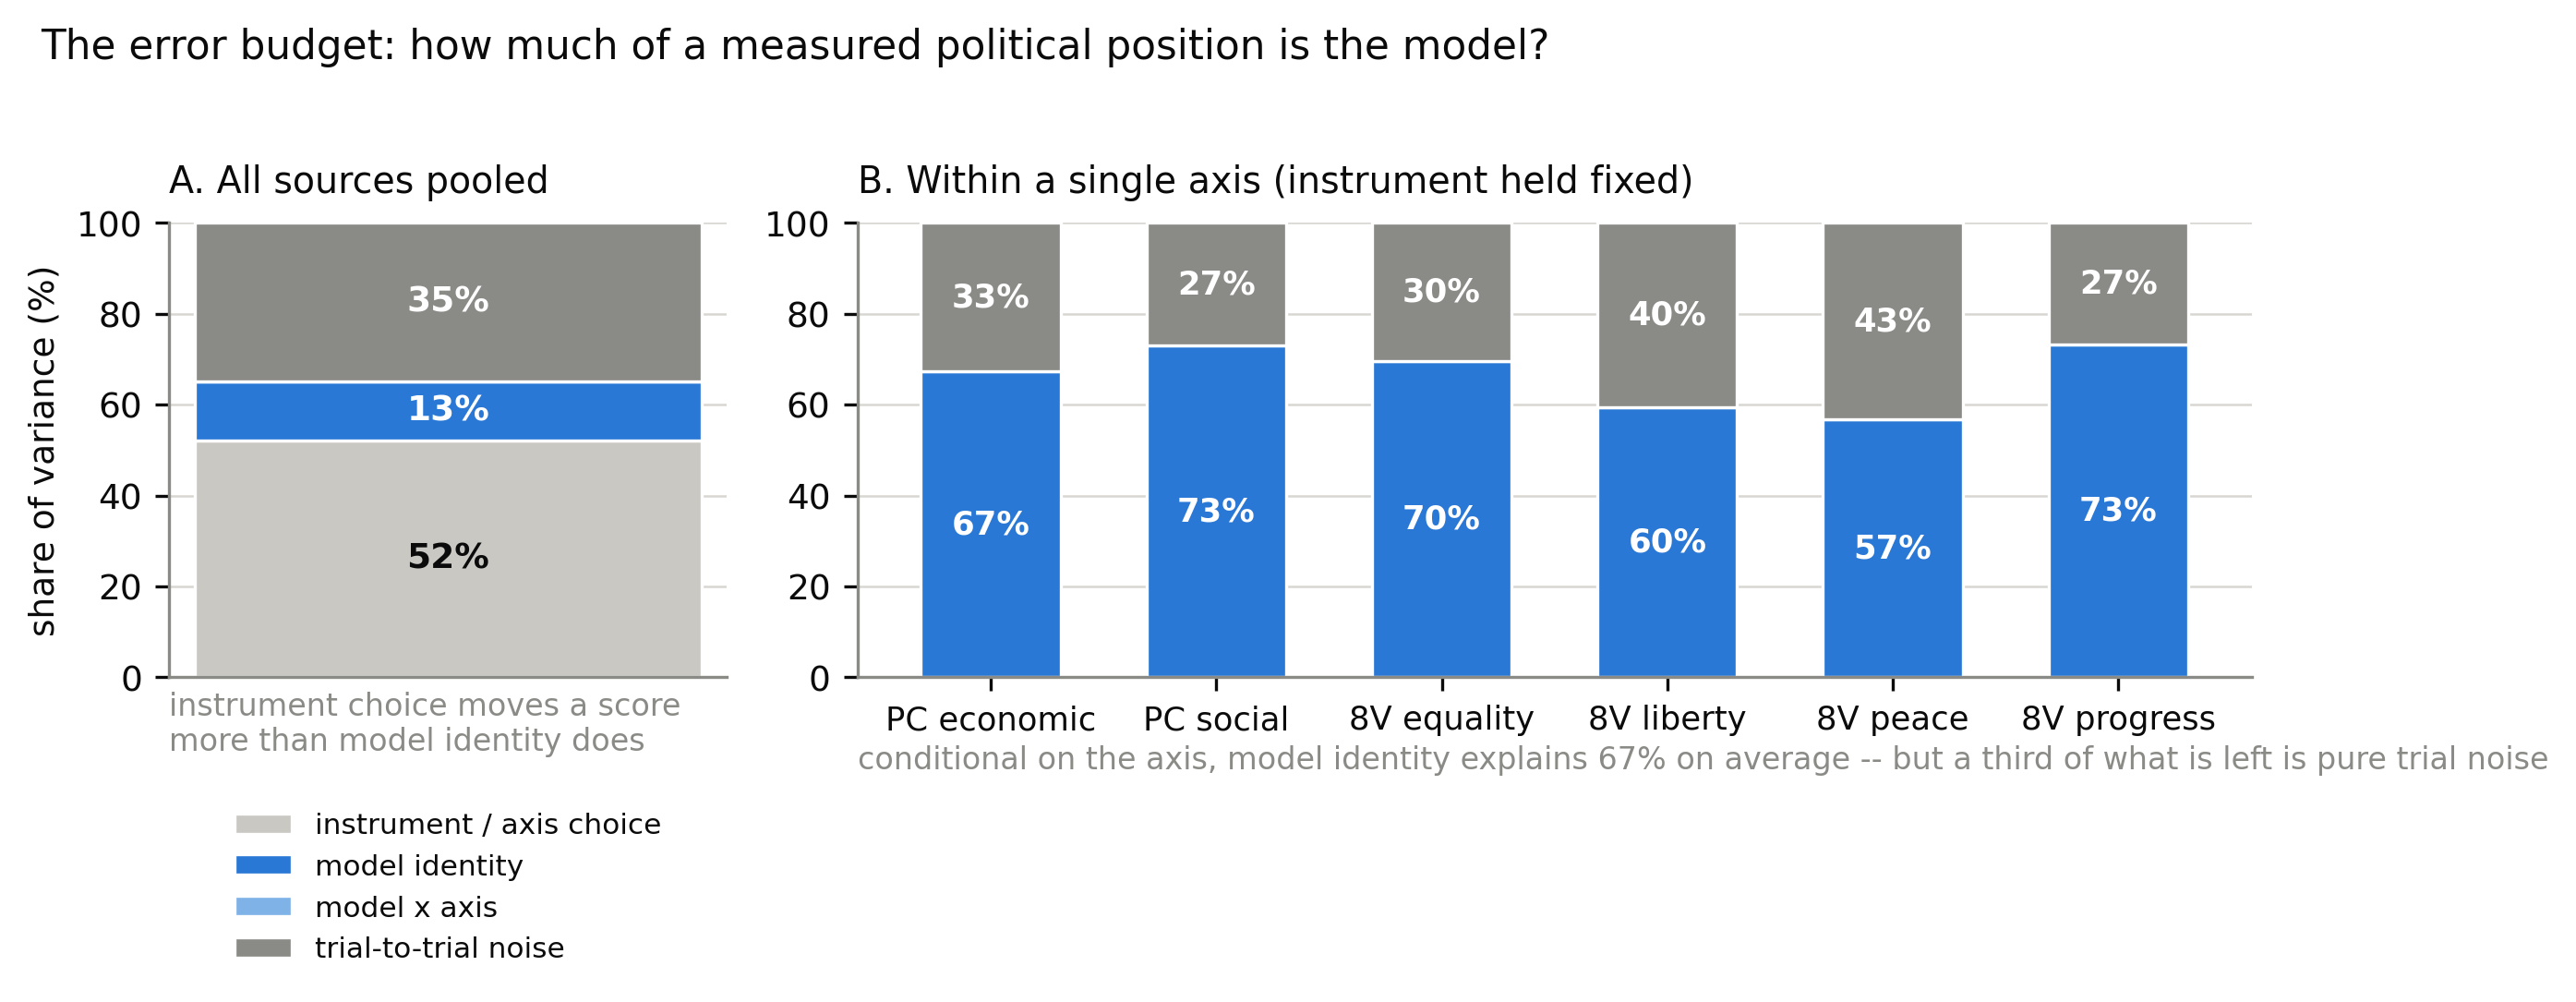
\includegraphics[width=\textwidth]{figures/fig6_error_budget.png}
\caption{\textbf{The error budget.} Variance components of a measured
political position, from a crossed random-effects model on 2,280
administrations. (\textbf{a}) Pooled across instruments: instrument and
axis choice accounts for 52\% of variance (95\% CI [35\%, 72\%]), model
identity for 13\% ([0.02\%, 22\%]), residual trial noise for 35\% ([19\%,
49\%]); cluster bootstrap over 19 models, 2,000 resamples.
(\textbf{b}) Within a single axis, where the between-instrument term is
removed by construction, model identity accounts for 57--73\%. Panel (a)
governs comparison across studies using different instruments; panel (b)
governs comparison within one study.}
\label{fig:error-budget}
\end{figure}

\begin{table}[H]
\centering
\caption{Every measurement factor examined explains more variance than
model identity does under the field's standard protocol. Model identity's
share is reported under whichever baseline each factor's own design used;
intervals are cluster bootstraps over models.}
\label{tab:factors}
\begin{tabular}{lp{4.6cm}p{4.6cm}r}
\toprule
Factor & Model identity & Factor itself & $n$ \\
\midrule
Instrument (2 instruments) & 13.0\% [0.02, 21.9] & 52.2\% [35.0, 71.9] & 2,280 \\
Instrument (4 instruments) & 1.89\% [0.0, 6.0] & --- & 8,640 \\
Asker identity & $\eta^2$ 0.56--0.73 (unattrib.) & $\eta^2$ 0.79 [0.65, 0.93] & 2,160 \\
Response format & $\eta^2$ 0.23 [0.04, 0.52] & $\eta^2$ 0.39 [0.02, 0.74] & 4,320 \\
Instrument contamination & --- & CI 0.046 [0.038, 0.055]; 17/18 models & 1,080 \\
\bottomrule
\end{tabular}
\end{table}

\subsection{Convergent and discriminant validity}
\label{sec:mtmm}

If instrument choice moves scores this much, the natural defence is that
both instruments are noisy measures of one underlying position. A
multi-trait multi-method analysis rejects this (Figure~\ref{fig:mtmm};
Table~\ref{tab:mtmm}). Convergent validity, the same construct measured by
both instruments, averages $r=-0.26$ across the 19 models. Discriminant
validity, different constructs measured by the same instrument, averages
$r=+0.52$. The Campbell--Fiske criterion requires the first to exceed the
second. Here the ordering is inverted and the convergent coefficient is
negative.

\begin{figure}[H]
\centering
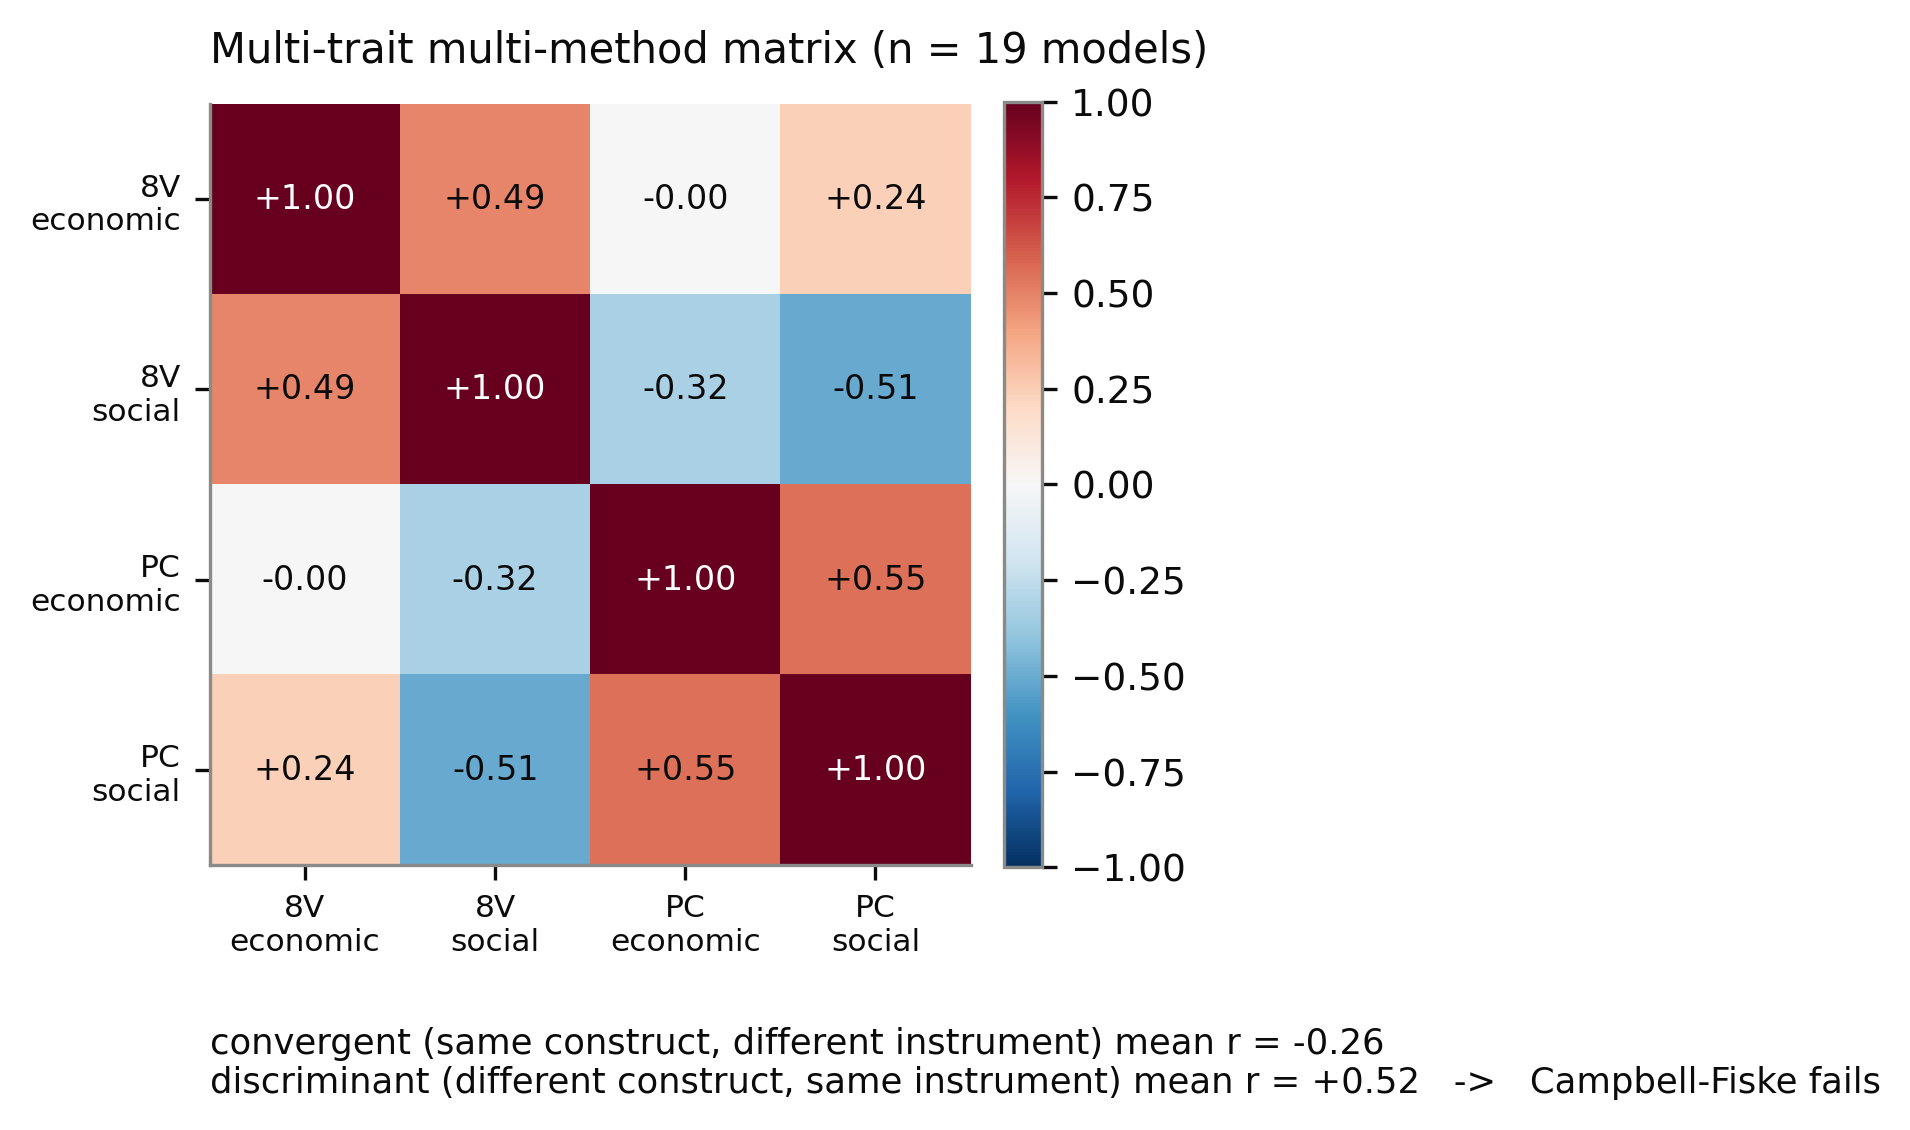
\includegraphics[width=0.7\textwidth]{figures/figSI_mtmm.png}
\caption{Multi-trait multi-method matrix across the 19 models. Convergent
coefficients (same construct, different instrument) average $r=-0.26$;
discriminant coefficients (different construct, same instrument) average
$r=+0.52$. The Campbell--Fiske ordering is inverted.}
\label{fig:mtmm}
\end{figure}

\begin{table}[H]
\centering
\caption{Multi-trait multi-method coefficients across the 19 models, each
with its standard error, $SE(r)=\sqrt{(1-r^2)/(n-2)}$, $n=19$.}
\label{tab:mtmm}
\begin{tabular}{llrr}
\toprule
Type & Pair & $r$ & $SE(r)$ \\
\midrule
Convergent & 8Values:economic vs. Pol.\ Compass:economic & $-0.005$ & 0.243 \\
Convergent & 8Values:social vs. Pol.\ Compass:social & $-0.506$ & 0.209 \\
Discriminant & 8Values:economic vs. 8Values:social & $+0.490$ & 0.211 \\
Discriminant & Pol.\ Compass:economic vs.\ Pol.\ Compass:social & $+0.549$ & 0.203 \\
\midrule
\textbf{Mean convergent} & & \textbf{$-0.255$} & \\
\textbf{Mean discriminant} & & \textbf{$+0.520$} & \\
\bottomrule
\end{tabular}
\end{table}

A model ranked as economically left by one instrument is, if anything,
ranked less so by the other. Separately, the four 8Values axes correlate
with each other at mean $r=0.71$ (liberty--peace, $r=0.85$), the signature
of one dominant general factor rather than four separable traits.

\subsection{Crossing four instruments}
\label{sec:four-instrument}

A preliminary check on SapplyValues partly replicates the directional
finding. All 18 models scored are economically left and culturally
progressive, but not libertarian: only 7 of 18 models score as
libertarian on its authority axis. Its economic axis disagrees with
Political Compass on model ranking ($\rho=-0.49$, 95\% CI [$-0.78,-0.04$])
while agreeing with 8Values' equality axis in the expected direction
($\rho=-0.53$, [$-0.87,-0.01$]). On Pew's 2026 Political Typology, 16 of 18
models classify left of centre; two, \texttt{deepseek/deepseek-chat} and
\texttt{x-ai/grok-4.20}, classify as \emph{Pragmatic and Polite Right}. The
ordinal Pew position does not correlate with either continuous instrument
at this sample size ($\rho=0.04$, [$-0.39,0.51]$; $\rho=-0.03$,
[$-0.55,0.54]$).

Crossing both new instruments into the same crossed random-effects model
used for the two-instrument budget above collapses the pooled
model-identity share further, to 1.89\% (8,640 administrations;
Table~\ref{tab:factors}). The collapse is driven by SapplyValues actively
disagreeing with Political Compass on model ranking, not by Pew's coarser
ordinal scale diluting the signal: adding SapplyValues alone drops the
model share to 0.49\%; adding Pew alone only to 8.21\%. That
per-instrument breakdown directly answers the objection this crossing
exists to pre-empt, that a variance component estimated from two
instruments is meaningless, by showing the collapse is not an artefact of
diluting a real signal with a weak instrument.

\subsection{Three further measurement factors}
\label{sec:three-factors}

Three further apparatus components, each demonstrated only in isolation in
the prior literature, are larger than the model term when measured
directly on the same 18 models (Table~\ref{tab:factors}). Framing the
asker's identity explains more variance ($\eta^2=0.79$, [0.65, 0.93]) than
model identity does under the field's standard unattributed condition
($\eta^2=0.56$--$0.73$); accommodation is asymmetric, moving scores
2.9--6.7 times further from baseline for a conservative framing than a
progressive one, on top of a baseline that already leans left. Sense-inverting
instrument items with the scoring key flipped produces a Contamination
Index averaging 0.046 ([0.038, 0.055]) of the instrument's own range, with
17 of 18 models shifting on at least one axis after Benjamini-Hochberg
correction; a companion memorisation probe (16 of 18 models parsed) finds a
16.6\% verbatim and 20.6\% near-verbatim completion rate. Free-text
elicitation, judged onto the same scale, versus a forced label explains
more variance (39\%, [0.02, 0.74]) than model identity within the same
design (23\%, [0.04, 0.52]).

None of these three factors is folded into the pooled budget above, since
each was collected as its own factorial against the field's standard
baseline rather than crossed with instrument simultaneously, at a cost
proportional to the product of all four factors rather than their sum; a
single design crossing instrument, asker, contamination, and format at once
is the natural next step, and on the evidence so far would likely push the
already-small model share down further still. That is the direction every
factor examined has pushed, and none has pushed the other way.

\subsection{Item-level reliability and IRT}
\label{sec:irt}

Measured per item rather than per axis, 44.8\% of model--item cells are
perfectly stable across all 60 repetitions, while the most volatile decile
of items carries under 16\% of total response entropy on either
instrument: inconsistency is concentrated in a minority of contested
items, not distributed evenly across a model's responses. A
range-normalized stability metric we previously reported in earlier work
normalised dispersion by each sample's own observed range, which assigns
one of the worst stability scores in the cohort to a model whose sixty
answers varied by six hundredths of a point on a twenty-point scale; we
report that failure explicitly here rather than quietly replacing it,
since any scale-free consistency statistic that divides by observed spread
inverts the same way on tightly clustered responses, and several published
consistency measures in this literature are constructed the same way.

A graded-response item-response-theory reanalysis of the same item-level
responses, separating response avoidance from ideological engagement,
tracks the published axis scores closely on five of the six axes
($\rho\geq0.86$); on 8Values, the model answering most items neutrally does
so roughly six times more often than the least avoidant model (52\% versus
9\% of items), consistent with some of the apparent centrism being
avoidance rather than moderation.

% =============================================================================
\section{Discussion}
% =============================================================================

The finding that language models lean left of centre is real in the sense
that it reproduces: we obtain it here on 19 models and two instruments, as
others have obtained it elsewhere. What this paper adds is a denominator.
When the measured quantity is decomposed, the instrument contributes four
times more variance than the model, and simple repetition of the same
measurement contributes more than twice as much. The lean survives, but the
\emph{magnitude} of a reported lean is mostly not about the model.

That distinction matters because the literature's quantitative claims are
magnitude claims. Statements that one model is more partisan than another,
that a provider's alignment procedure shifts a model's politics by some
amount, or that lean has grown or shrunk across model generations, all
require that scores be comparable across studies. Our MTMM result says they
are not: the two most widely used instruments produce negatively
correlated rankings of the same construct across the same models. Pooling
or contrasting scores obtained with different instruments is therefore not
a conservative approximation; it is an operation with no defined meaning.

We want to be precise about the scope of this claim, because it is easy to
overstate. We are not arguing that political-bias audits are uninformative,
nor that the models are politically neutral, nor that any particular
published paper is wrong. Within a single study using a single instrument,
model identity is clearly measurable and accounts for roughly two-thirds of
the remaining variance; rank orderings obtained that way are meaningful.
The failure is one of transportability. It also has a straightforward
remedy: report the apparatus alongside the estimate rather than the
estimate alone. That remedy has precedent in this journal specifically. A
study using ChatGPT to approximate ANES responses, discussed in Section 2.1
above, and a study evaluating LLMs' zero-shot fidelity to human-written
codebooks for political-text coding \citep{halterman2025codebook}, reach
structurally similar conclusions for two different LLM measurement tasks.
Across three independent lines of work on three different measurement
tasks, published in this journal within about two years, none finds an
off-the-shelf LLM output safe to treat as a measurement without
characterizing how it fails.

Nor are we claiming that a questionnaire score predicts what a model would
do given a real decision. A dual-instrument study comparing an abstract
voting-advice questionnaire against real referendum outcomes finds that the
two disagree: models cluster near the political centre on concrete votes
despite a left-leaning profile on the questionnaire, and at least part of
the questionnaire signal may reflect change-aversion rather than ideology
\citep{barmettler2026instrument}. That is a claim about behavioural
validity, which this design does not test and does not need to in order
for the instrument-comparability problem above to hold; an error budget for
a questionnaire score is not an argument that the score predicts behaviour,
and the two questions call for different studies.

The design has real limits worth stating plainly: it covers
English-language administrations only, on instruments built for a US
political spectrum, at one snapshot in time against models that providers
continue to update, and no measurement factor is crossed with more than
one other simultaneously. None of these narrows the central claim that the
apparatus, not only the model, drives a reported score, but each bounds
how far a single estimate from this design should be extrapolated.

\subsection*{A minimum reporting standard for political-bias audits}

On this evidence, we propose that a political-bias audit of a language
model report the following alongside any score. \emph{The instrument,
named, with its items}: scores from different instruments are not on a
common scale and should not be compared numerically. \emph{The asker
condition}, including the absence of one: an unattributed prompt is a
condition, not a neutral baseline. \emph{Repetition count and dispersion},
in the instrument's own units: trial noise here exceeded the model effect.
\emph{An error budget, or at minimum a variance decomposition} across
whatever was varied: a point estimate without a denominator cannot be
compared to another study's point estimate. \emph{A contamination check}
for instruments that appear in pretraining corpora. \emph{Item-level
results}, or at least the dispersion across items, since aggregate
stability scores conceal that inconsistency concentrates in a minority of
contested items. Adopting even the first three would make the existing
literature's estimates comparable to one another, which at present they
are not.

% =============================================================================
\section*{Funding}
% =============================================================================

The author received no specific funding for this work.

% =============================================================================
\section*{Acknowledgements}
% =============================================================================

Portions of this manuscript's text were drafted and revised with the
assistance of a commercial AI writing assistant, used interactively by the
author throughout the project's development in 2026, accessed via a paid
subscription. Portions of the data-collection pipeline, scoring adapters,
and statistical-analysis scripts were developed with the assistance of a
commercial AI coding assistant, used the same way; every script, formula,
and output produced this way was reviewed and independently verified by
the author before use, including an independent reproduction of the
four-instrument variance-components result from raw data in a clean
environment. The author directed all content and analysis decisions,
verified all reported numbers against the underlying data and code, and
takes full responsibility for the manuscript's content and claims.

% =============================================================================
\section*{Data Availability Statement}
% =============================================================================

All raw per-trial data, scoring adapters, and analysis code are released at
\url{https://github.com/sletch1/AI-Political-Bias-Research-Paper}, with a
submission-time snapshot archived at
\url{https://doi.org/10.5281/zenodo.22968158}. Full methods, the complete
four-instrument crossing, and the item-response-theory, prompt-robustness,
and open-ended-generation checks that corroborate the results above are in
the web appendix, submitted as supplementary material alongside this
manuscript. Replication materials will be deposited to the Political
Analysis Dataverse upon conditional acceptance.

% =============================================================================
\section*{Competing Interests}
% =============================================================================

Competing interests: the author declares none.

% =============================================================================
\section*{Ethics Declarations}
% =============================================================================

This study did not involve human participants, human data, or animal
subjects. All data consist of text outputs generated by third-party large
language models accessed via a commercial API (OpenRouter); no personal,
sensitive, or identifiable information is involved. Institutional ethics
review was therefore not required.

One instrument, Pew Research Center's 2026 Political Typology (Section
2.3), was scored by programmatically driving Pew's live public quiz and
reading off its own classification, rather than reimplementing Pew's
unpublished clustering procedure, following the same approach already used
for Political Compass. Reusing the instrument's item text and published
group definitions for research is covered by Pew's general terms of use.
Submitting the interactive quiz itself 180 times in an automated fashion is
a distinct question: it plausibly exceeds ordinary personal use of that
interactive tool, even though it accesses no respondent microdata or
personal information at any point. We disclose this explicitly rather than
treating it as settled by the terms-of-use analysis for the survey items.

% =============================================================================
\clearpage
\bibliographystyle{chicago}
\bibliography{references}

\end{document}
